\section{PROJECT DESCRIPTION}

\subsection{\underline{Reference Algorithm}}
Vortex recommendation module follows a hybrid content-driven approach: 

\begin{itemize}
    \item \textbf{Content Similarity}
    \begin{itemize}
        \item TF-IDF vectorization performed over game metadata (genres, themes, and descriptions).
        \item Cosine similarity calculation between candidate games and user-liked titles.
    \end{itemize}

    \item \textbf{Preference Adjustment}
    \begin{itemize}
        \item Conversion of binary feedback (Like/Dislike) into a weighted preference score.
    \end{itemize}

    \item \textbf{Mood Adjustment}
    \begin{itemize}
        \item Encoding of user-selected moods using one-hot vectors.
        \item Application of a mood-genre mapping to modify candidate scores dynamically.
    \end{itemize}

    \item \textbf{Final Rank}
    \begin{itemize}
        \item Weighted aggregation of similarity, preference, quality, and an exploration factor.
    \end{itemize}
\end{itemize}

Note: The current Python implementation is a work-in-progress with known suggestion inaccuracies; calibration and validation are ongoing.


\subsection{\underline{Characteristic of Data}}

Vortex utilizes a combination of local behavioral data and external game metadata to power its recommendation engine and library management features. The dataset is characterized by a mix of categorical, numerical, text-based, and temporal information.

\paragraph{Primary and Secondary Sources}

\begin{description}

\item[\textbf{Primary Data Sources}]
The primary dataset is generated locally through user interactions with the launcher. This includes detected local game states (Game Name, Version, Install Directory) and continuously produced behavioral metrics (Session Start/End times, Idle/Inactive duration, total Session length, Mood Session IDs, and explicit Liked/Disliked Games).

\item[\textbf{Secondary Data Sources}]
The secondary dataset is sourced externally from the Internet Game Database (IGDB) and digital distribution APIs. IGDB provides rich, structured JSON metadata via a REST API, contributing Genre/Tags, Game Length, Developer/Publisher details, and Ratings/Reviews. Additional platform-specific data, such as in-game achievements, is retrieved from APIs like Steam's.

\end{description}

\paragraph{Sampling Techniques}

Data collection relies on real-time event capture rather than traditional batch data sampling. User actions and session logs are continuously recorded as raw events and stored dynamically in the local SQLite database. External metadata is not sampled from a static database dump; instead, it is fetched dynamically via HTTP POST requests to the IGDB API as needed, strictly governed by a rate limit of 4 requests per second.

\paragraph{Statistical Methods and Data Processing}

The system employs several statistical and machine learning techniques to process and quantify raw data for the recommendation pipeline:

\begin{description}

\item[\textbf{One-Hot Encoding}]
Applied to convert categorical data—such as game genres and user moods (e.g., ``Relaxed'', ``Competitive'')—into a binary numerical format for model processing.

\item[\textbf{TF--IDF Vectorization}]
(Term Frequency – Inverse Document Frequency) is used to process unstructured text documents, such as game descriptions, converting them into multi-dimensional numerical float vectors.

\item[\textbf{Normalization}]
Continuous variables, such as total playtime duration and external review ratings (e.g., Metacritic scores), are scaled and normalized to float values between 0.0 and 1.0 to ensure uniform weight distribution in the ranking algorithm.

\item[\textbf{Cosine Similarity}]
Utilized within the content-based filter to mathematically determine the distance and similarity between the TF--IDF feature vectors of candidate games and those the user has positively rated.

\item[\textbf{Weighted Aggregation}]
The Hybrid Ranker calculates a final recommendation score by applying mathematical weights to various quantified inputs: Preference Match (0.40), Similar to Liked Games (0.35), Quality Score (0.15), and an Exploration Factor (0.10) to output a final percentage-based rank.

\end{description}

\subsection{\underline{SWOT Analysis}}
\begin{itemize}
    \item \textbf{Strengths}
    \begin{itemize}
        \item Unified launcher concept providing practical utility for game management.
        \item High-performance execution leveraging native C++.
        \item Extendable architecture designed for future machine learning evolution.
    \end{itemize}
    \item \textbf{Weaknesses}
    \begin{itemize}
        \item Inconsistent recommendation quality in the current iteration.
        \item Partial integration between the C++ core and Python modules.
        \item User Interface is not yet finalized in its intended QML form.
    \end{itemize}
    \item \textbf{Opportunities}
    \begin{itemize}
        \item Integration of additional platforms such as GOG and Epic Games.
        \item Enhancement of recommendation logic through feature engineering and model tuning.
        \item Positioning as a lightweight alternative to resource-heavy game launchers.
    \end{itemize}
    \item \textbf{Threats}
    \begin{itemize}
        \item Potential API changes or rate limits from external services like Steam and IGDB.
        \item Data sparsity issues, specifically regarding the "cold start" problem for new users.
        \item Risk of scope creep within the constraints of the academic timeline.
    \end{itemize}
\end{itemize}

\subsection{\underline{Project Features}}
\begin{itemize}
    \item \textbf{Multi-source Game List}: Integration of both Steam and local directory scanning.
    \item \textbf{Direct Launch}: Ability to initialize games directly from the Vortex interface.
    \item \textbf{Heuristic Filtering}: Basic exclusion of non-game executables during the directory scanning process.
    \item \textbf{Interactive Navigation}: Sorting and selection capabilities via an interactive menu.
    \item \textbf{Planned Features}: Implementation of analytics dashboards and mood-based recommendation displays.
\end{itemize}

\begin{figure}[H]
    \centering
    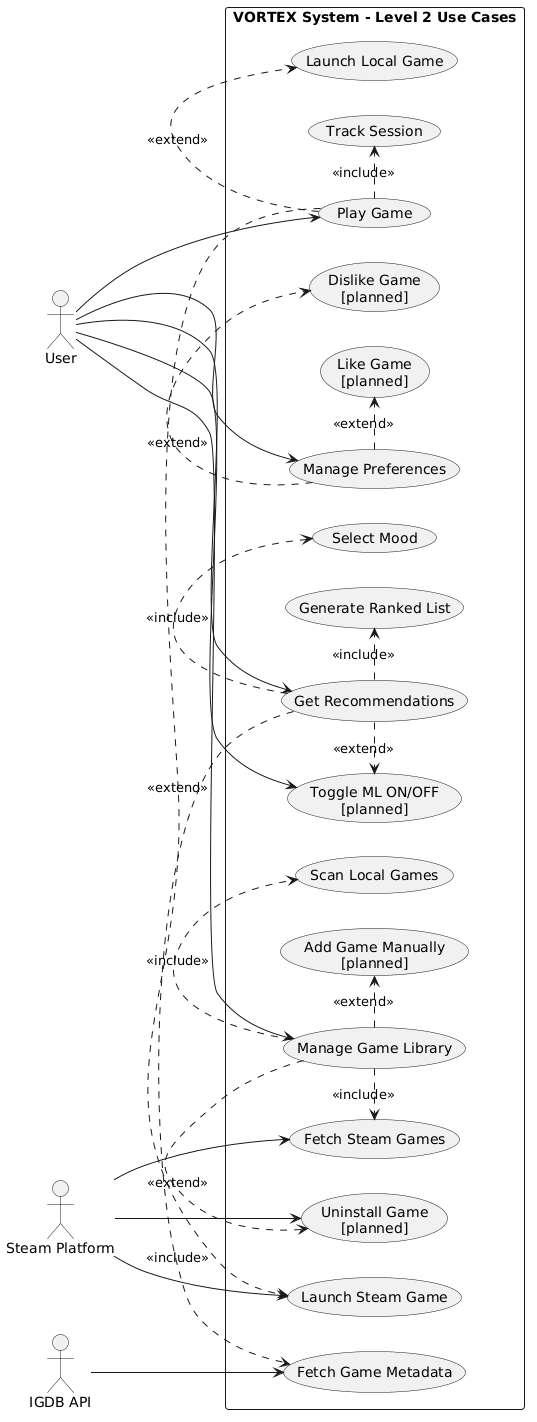
\includegraphics[height=1.5\textwidth]{../figures/level2 usecase diagram.png}
    \caption{Use Case Diagram Level-2 (Source: By Team)}
\end{figure}

\subsection{\underline{User Classes and Characteristics}}
\begin{itemize}
    \item \textbf{End User (Gamer)}
    \begin{itemize}
        \item Possesses basic technical knowledge.
        \item Requires a simple interaction model and low-latency system responses.
    \end{itemize}
    \item \textbf{Project Developer}
    \begin{itemize}
        \item Responsible for core modules (C++, Python, Database, and UI).
        \item Requires modular, decoupled, and testable components for iterative development.
    \end{itemize}
    \item \textbf{Evaluator / Faculty}
    \begin{itemize}
        \item Reviews the technical methodology, system architecture, and requirement traceability.
        \item Validates the alignment between project goals and final implementation.
    \end{itemize}
\end{itemize}



\subsection{\underline{Design and Implementation Constraints}}
\begin{itemize}
    \item \textbf{Primary OS Target}: System is specifically designed for the Windows operating system.
    \item \textbf{Steam Data Dependencies}: Retrieval relies on access to the Windows Registry and the local Steam file structure.
    \item \textbf{Local Discovery}: Local scanning logic currently assumes executable-based discovery targeting \texttt{.exe} files.
    \item \textbf{Recommendation Constraints}: Quality is contingent upon the completeness of metadata and the depth of available user history.
    \item \textbf{Temporal Constraints}: Project development is limited to a 12-week academic implementation window.
\end{itemize}

\newpage
\subsection{\underline{Design Diagrams}}
% \begin{figure}[H]
%     \centering
%     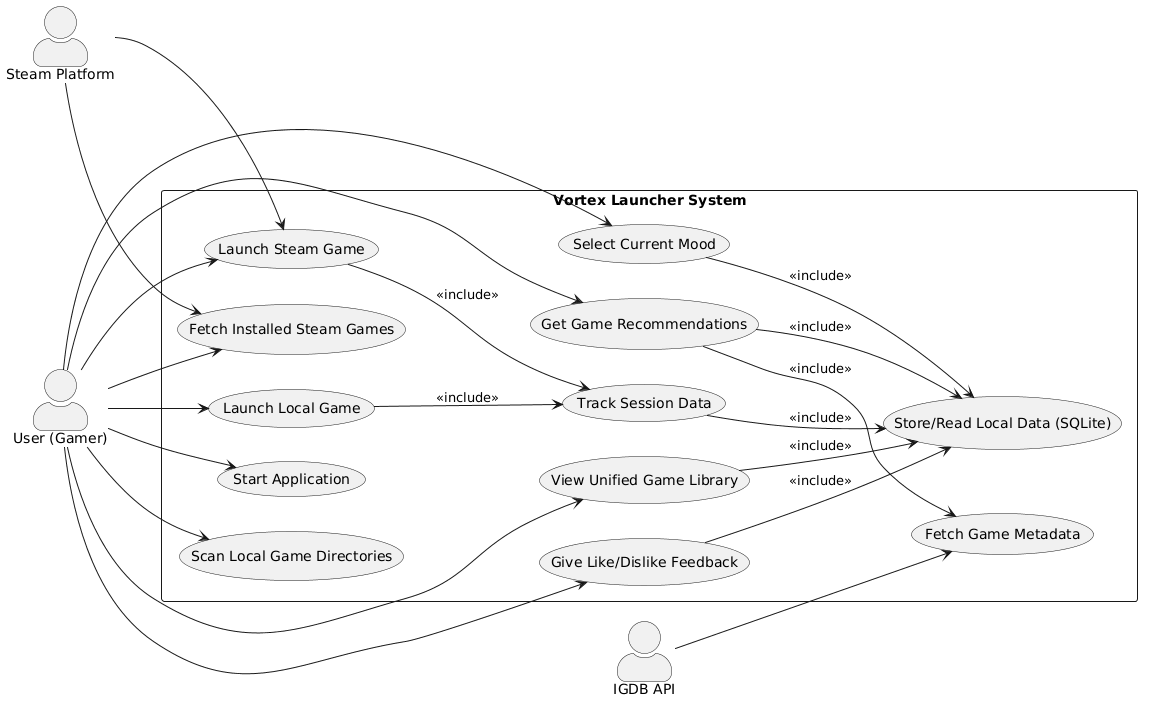
\includegraphics[width=0.75\textwidth,keepaspectratio]{../figures/usecase diagram.png}
%     \caption{Use Case Diagram}
% \end{figure}

\begin{figure}[H]
    \centering
    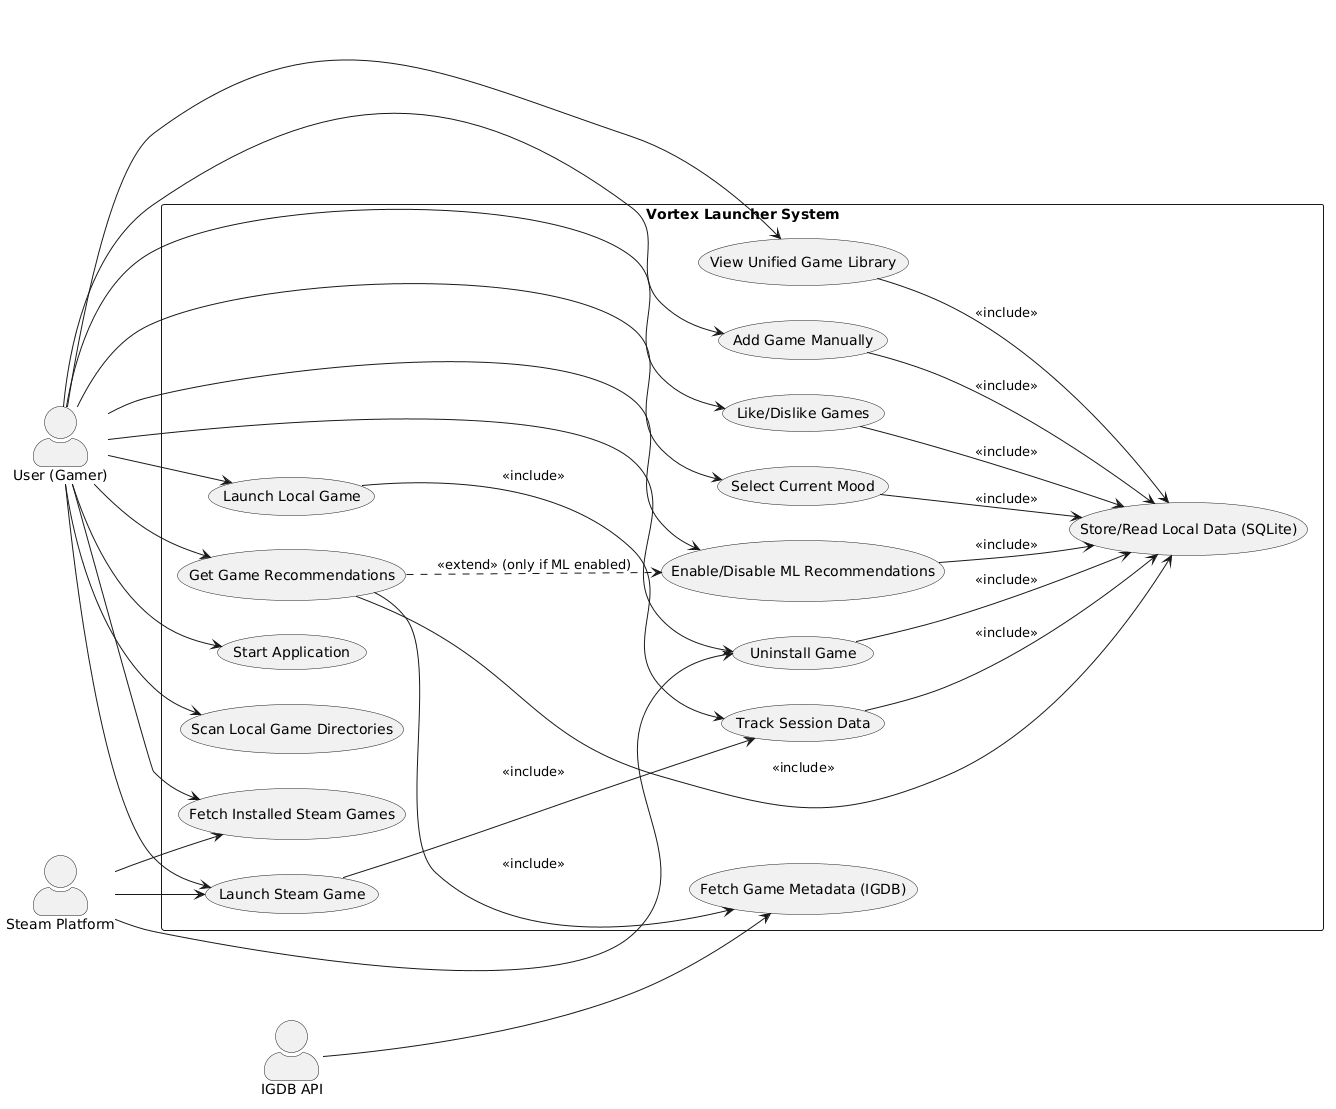
\includegraphics[angle=90, width=\textwidth, keepaspectratio]{../figures/usecase_diagram2.png}
    \caption{Use Case Diagram (Source: By Team)}
\end{figure}

\begin{figure}[H]
    \centering
    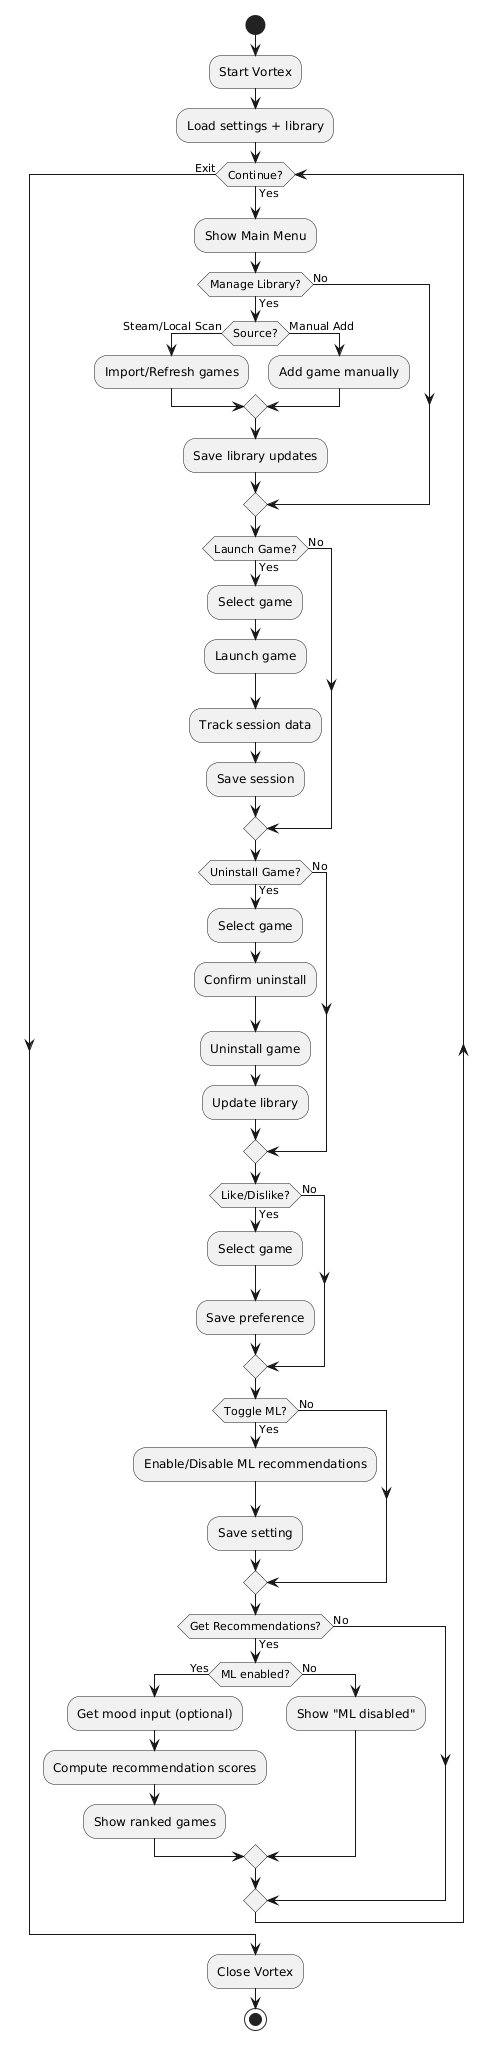
\includegraphics[height=\textheight,keepaspectratio]{../figures/ActivityDiagram_compact.png}
    \caption{Activity Diagram (Source: By Team)}
\end{figure}

% \begin{figure}[H]
%     \centering
%     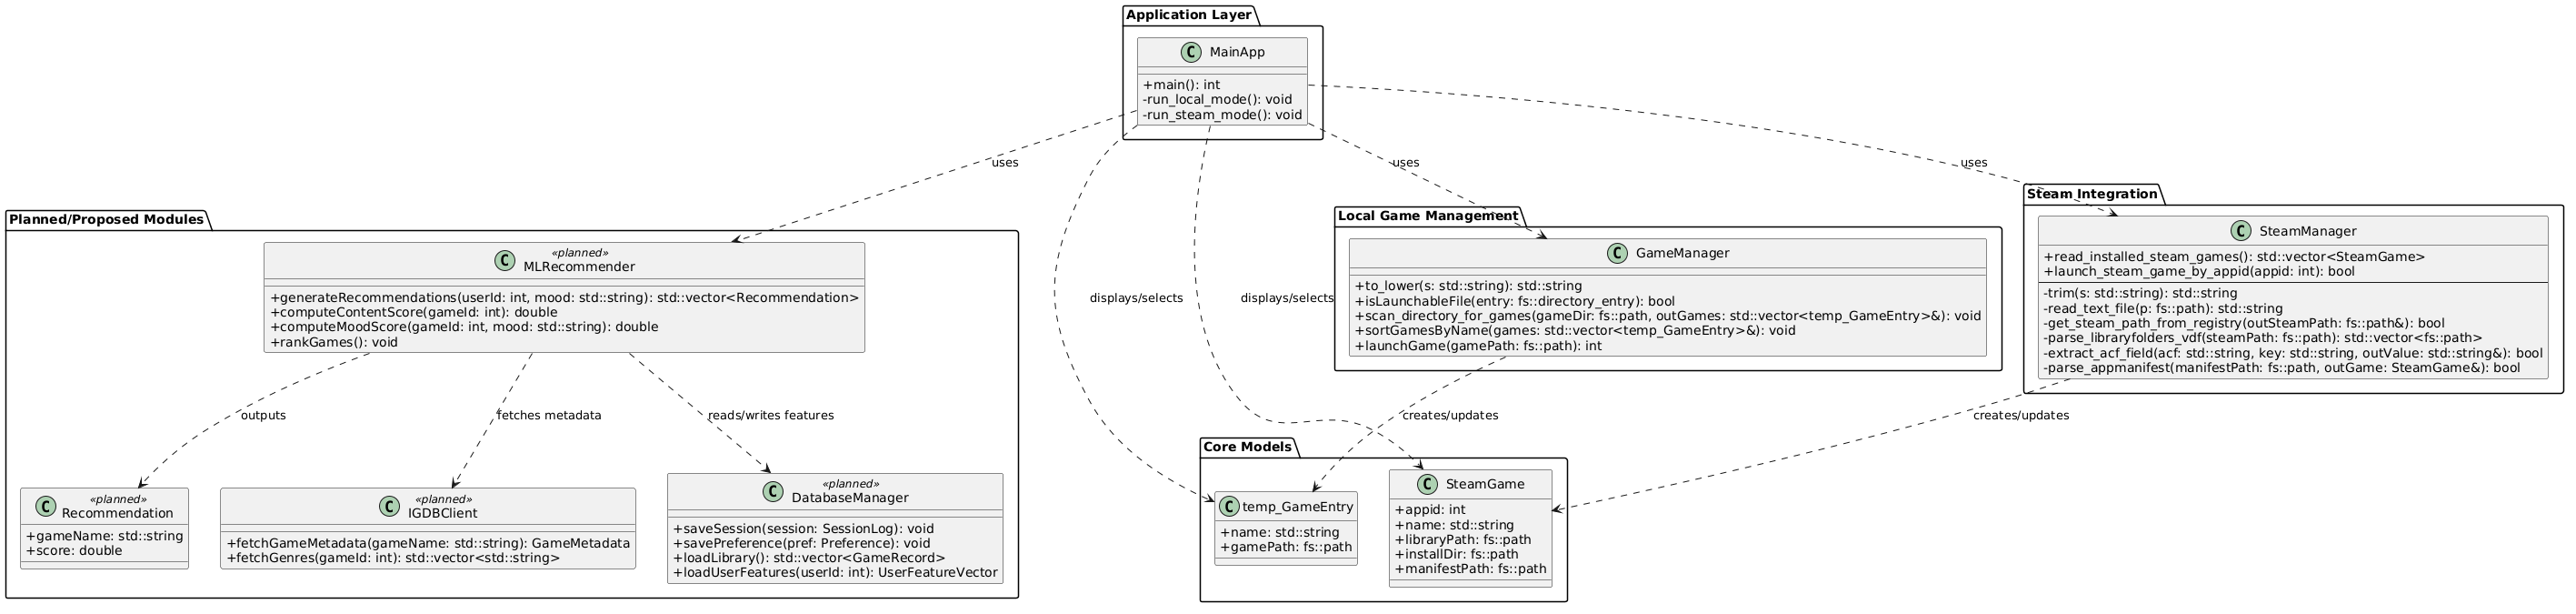
\includegraphics[width=0.9\textwidth]{../figures/class diagram.png}
%     \caption{Class Diagram}
% \end{figure}

\begin{figure}[H]
    \centering
    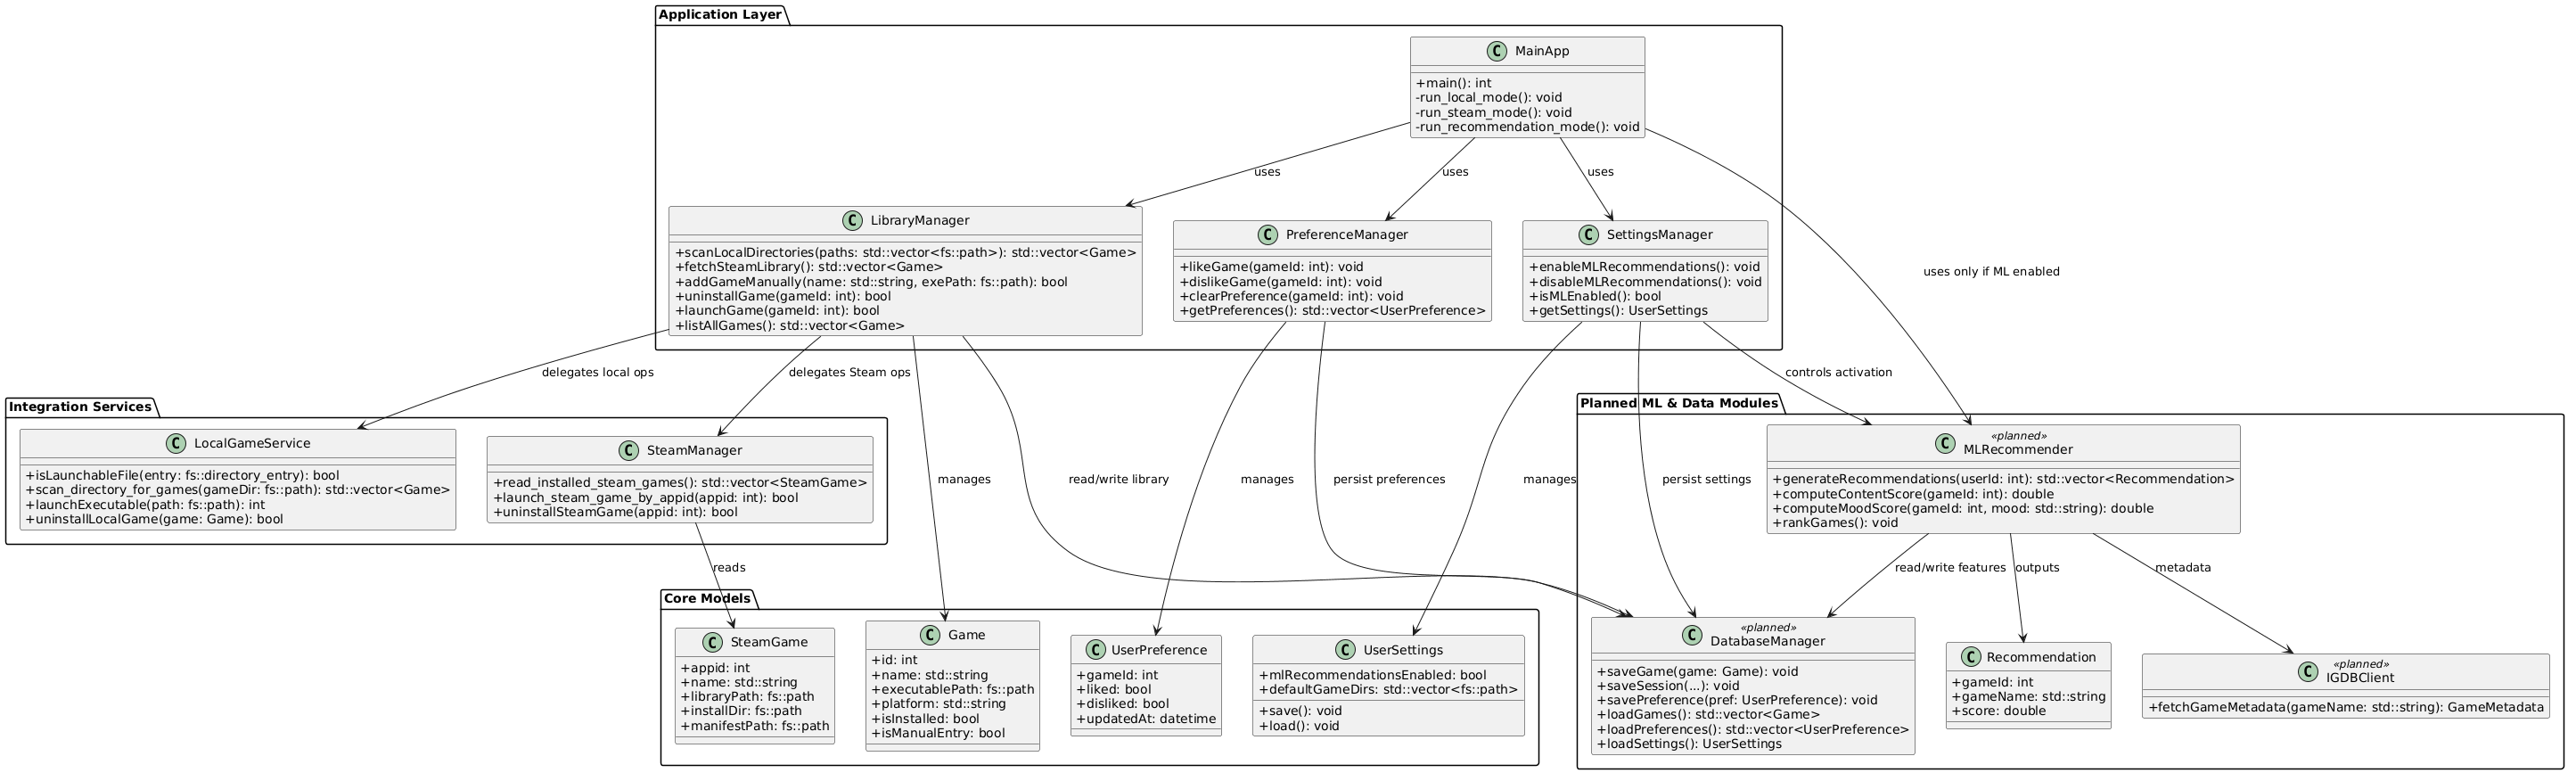
\includegraphics[angle=90, width=0.5\textwidth]{../figures/class_diagram2.png}
    \caption{Class Diagram 2 (Source: By Team)}
\end{figure}

\begin{figure}[H]
    \centering
    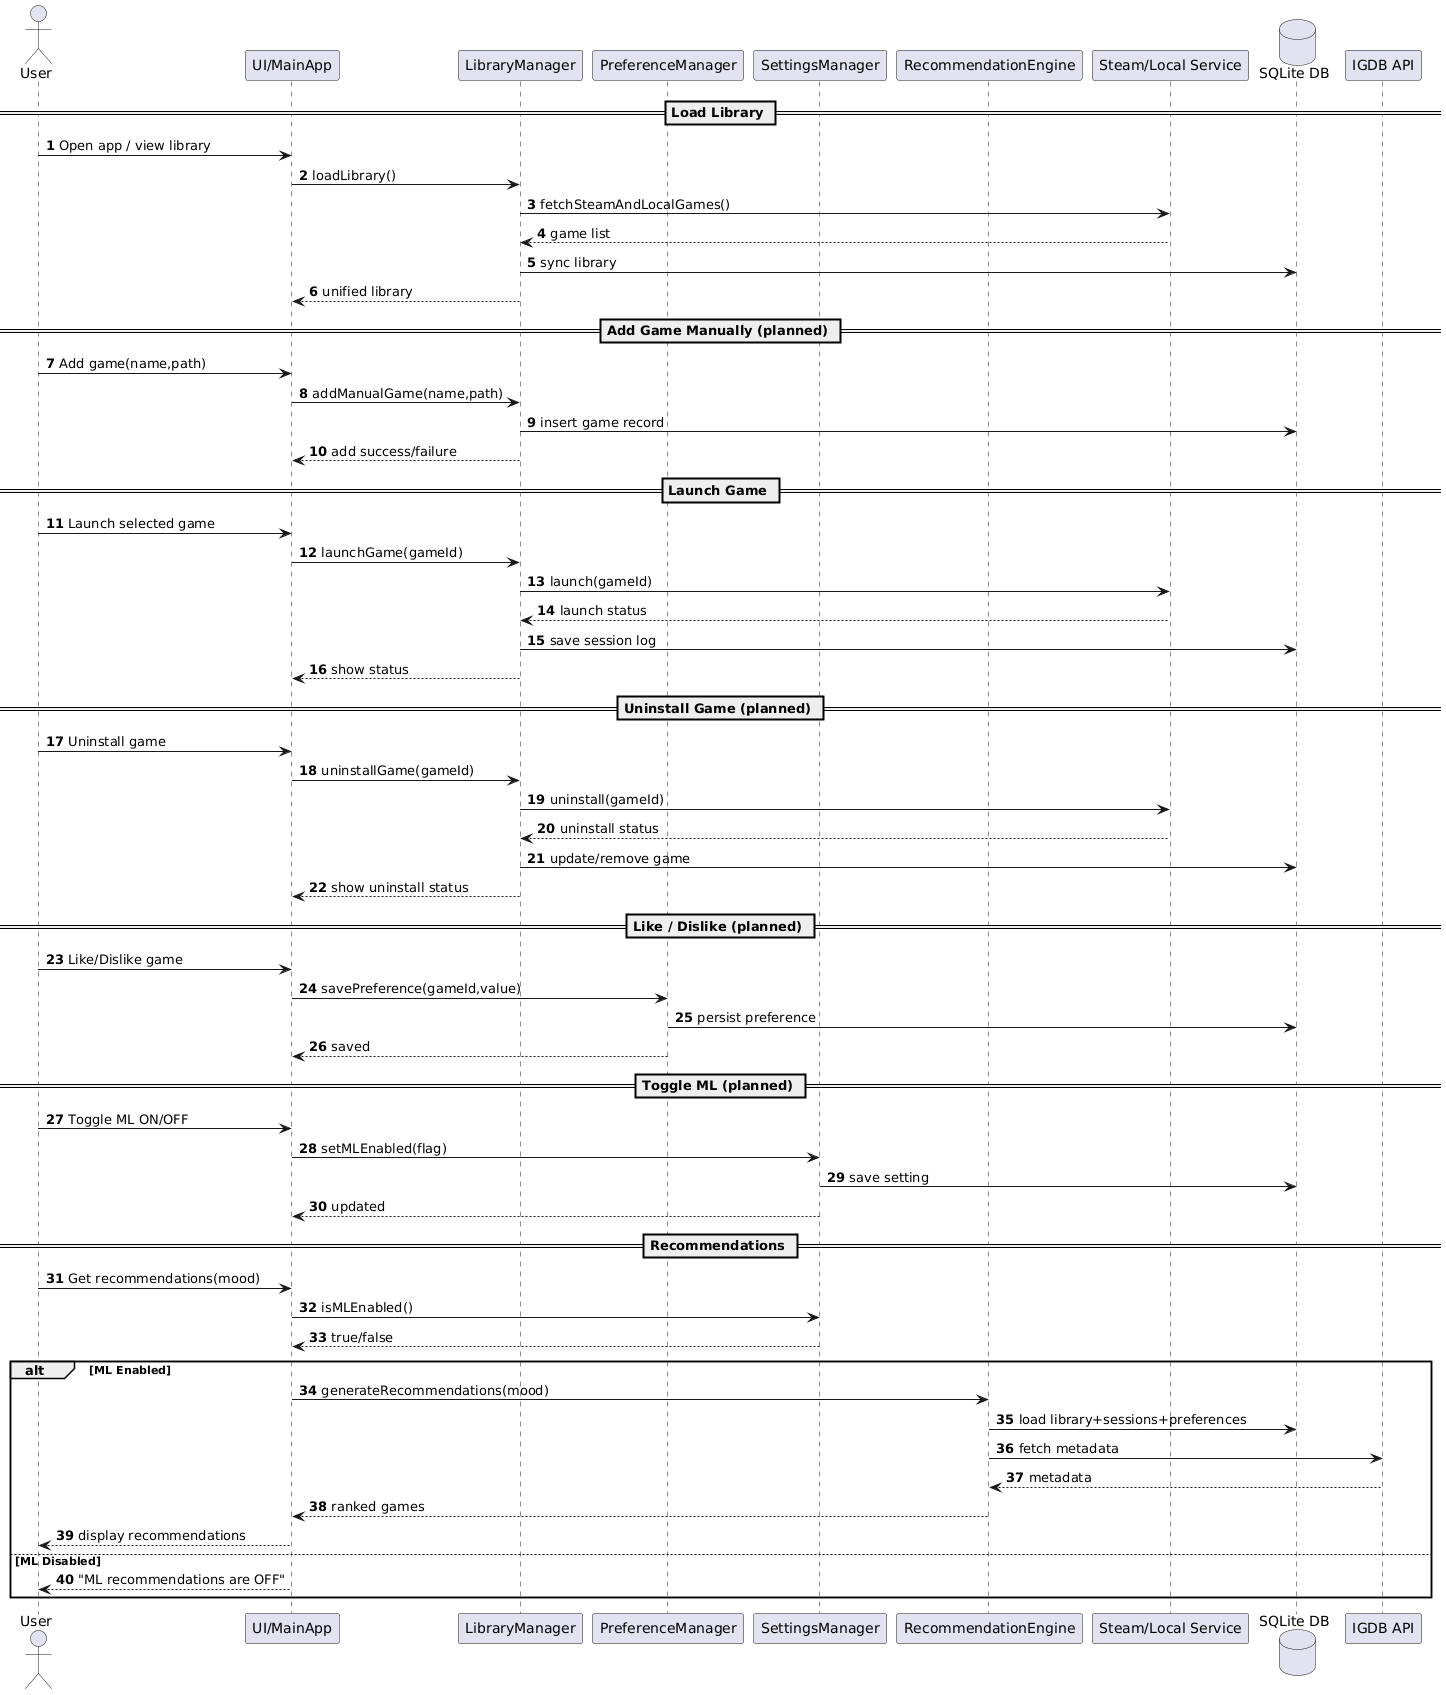
\includegraphics[width=\textwidth]{../figures/Sequence Diagram.png}
    \caption{Sequence Diagram (Source: By Team)}
\end{figure}

\begin{figure}[H]
    \centering
    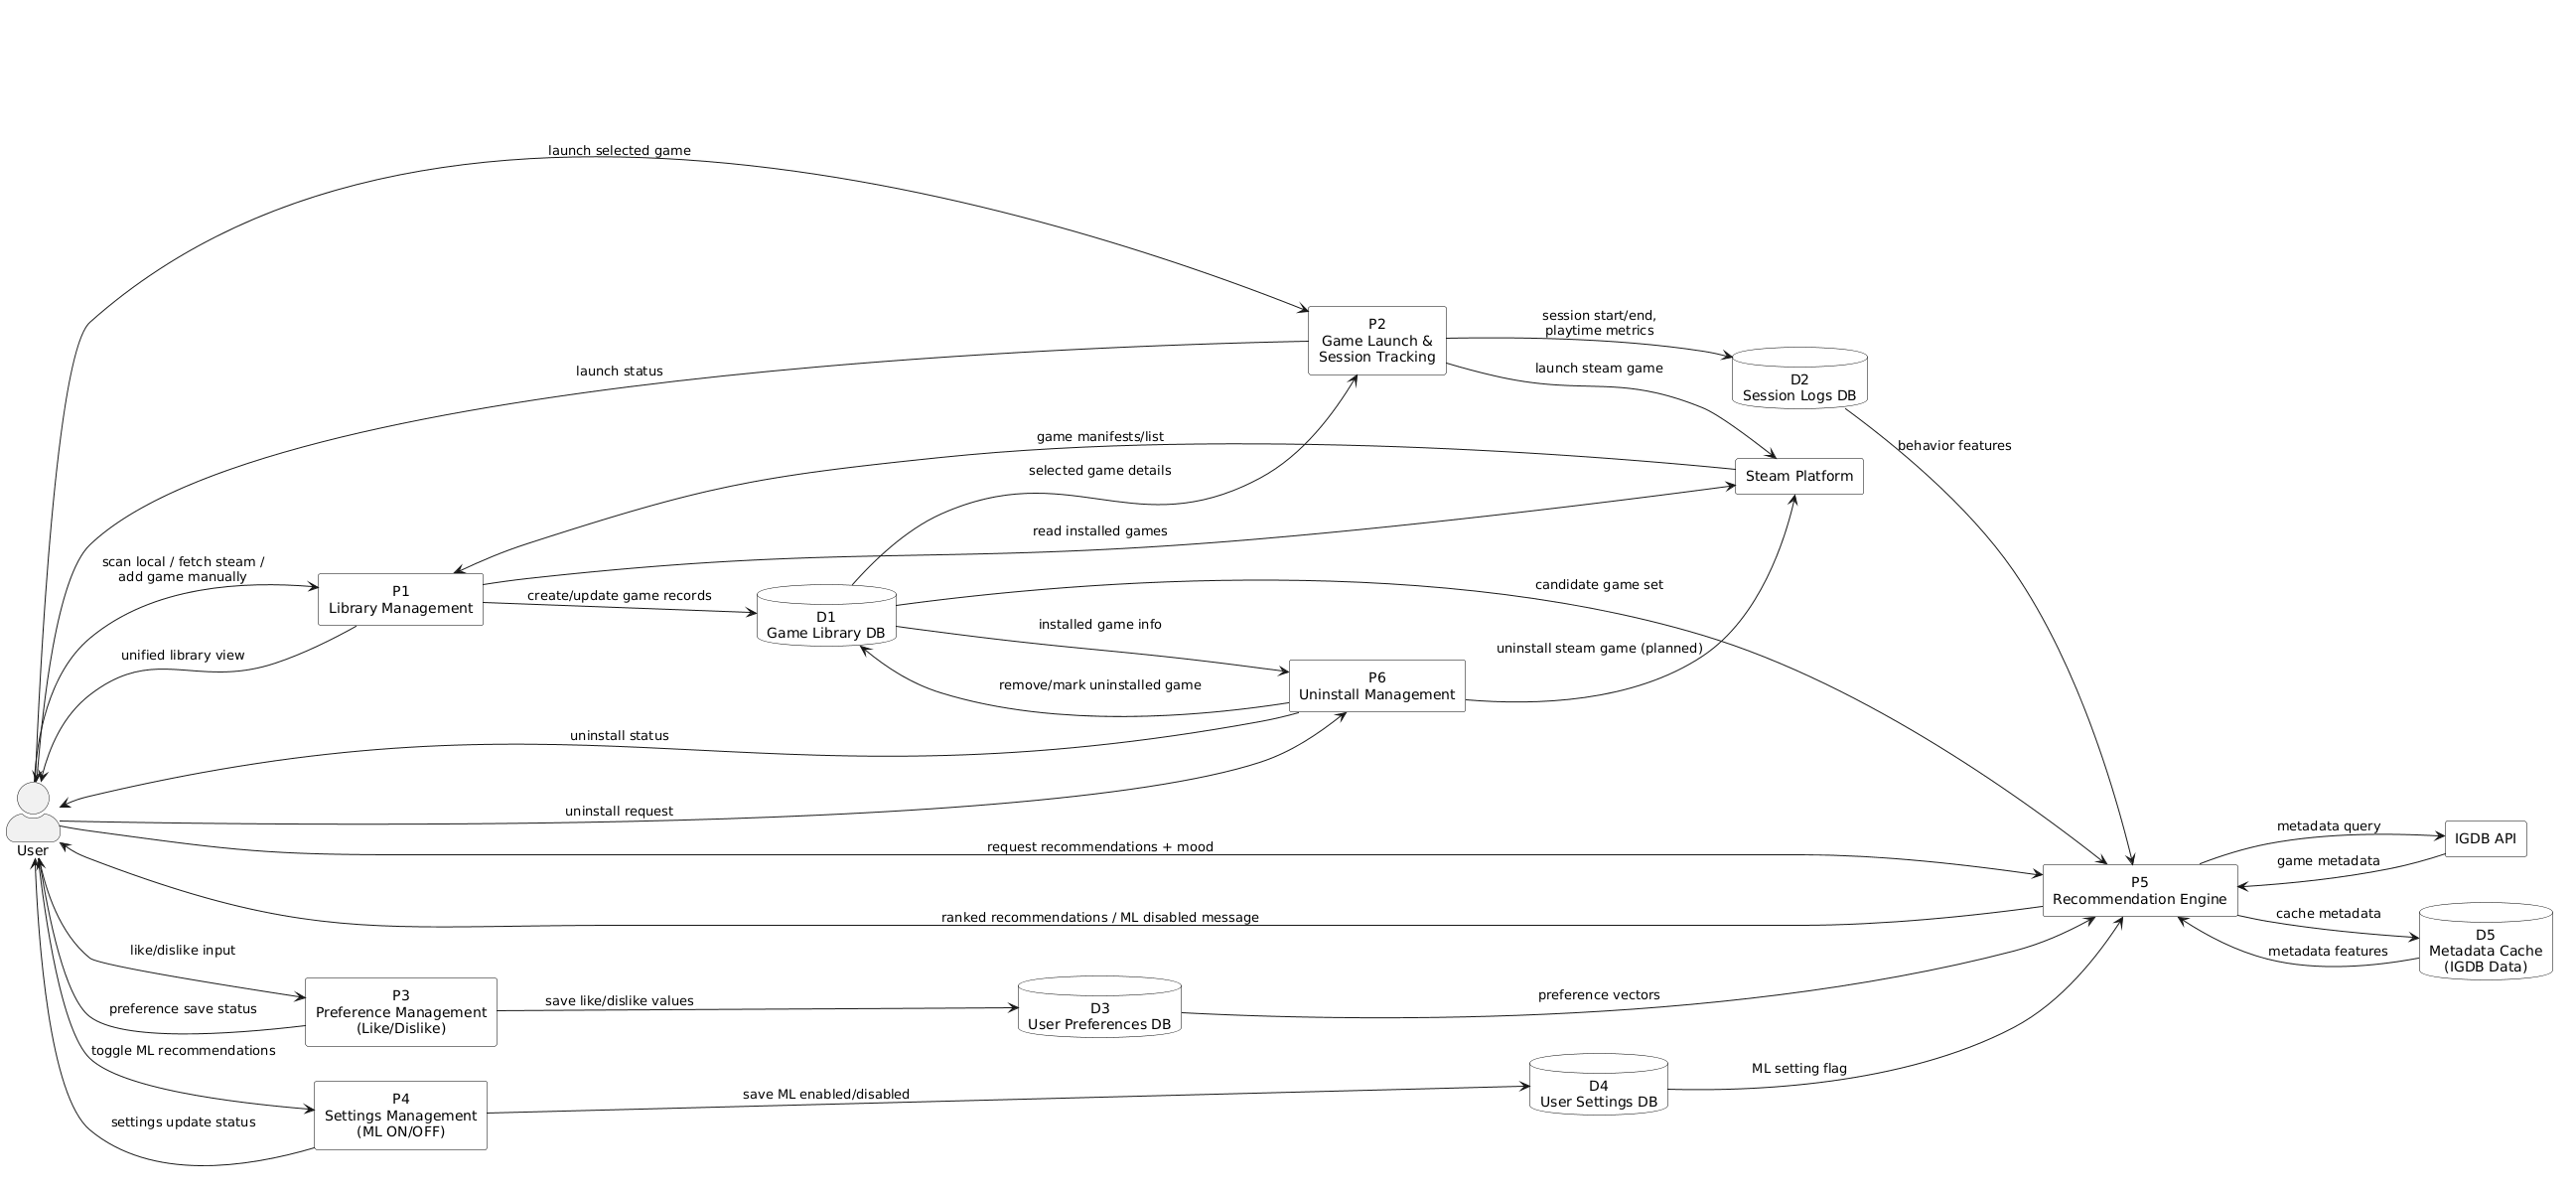
\includegraphics[angle=90, width=0.75\textwidth]{../figures/DFD.png}
    \caption{Data Flow Diagram (Source: By Team)}
\end{figure}

\begin{figure}[H]
    \centering
    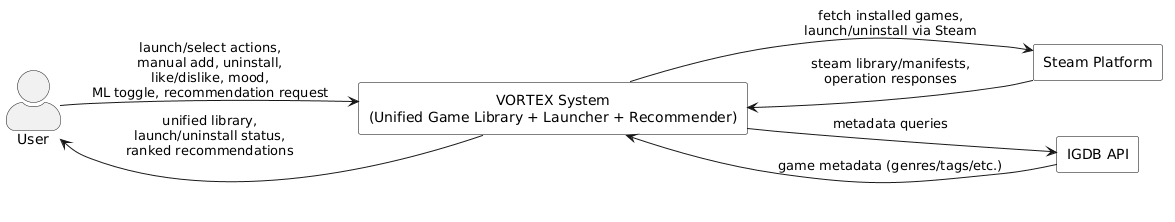
\includegraphics[angle=90, height=1.5\textwidth]{../figures/DFD level-0.png}
    \caption{Data Flow Diagram Level-0 (Source: By Team)}
\end{figure}

% \begin{figure}[H]
%     \centering
%     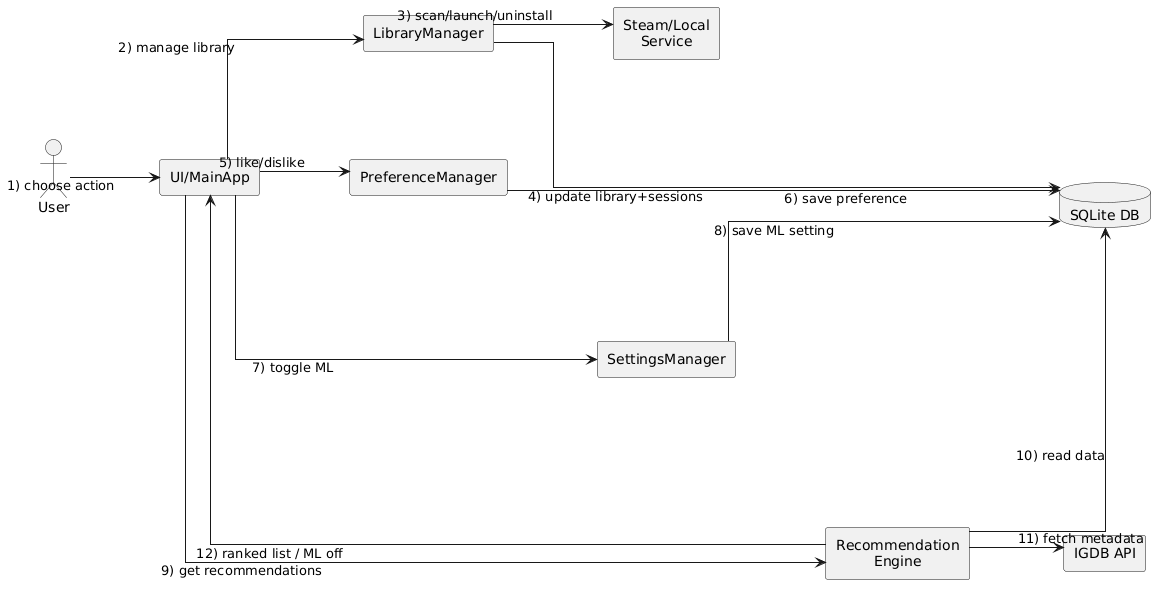
\includegraphics[width=0.8\textwidth]{../figures/Collaboration Diagram.png}
%     \caption{Collaboration Diagram}
% \end{figure}

\begin{figure}[H]
    \centering
    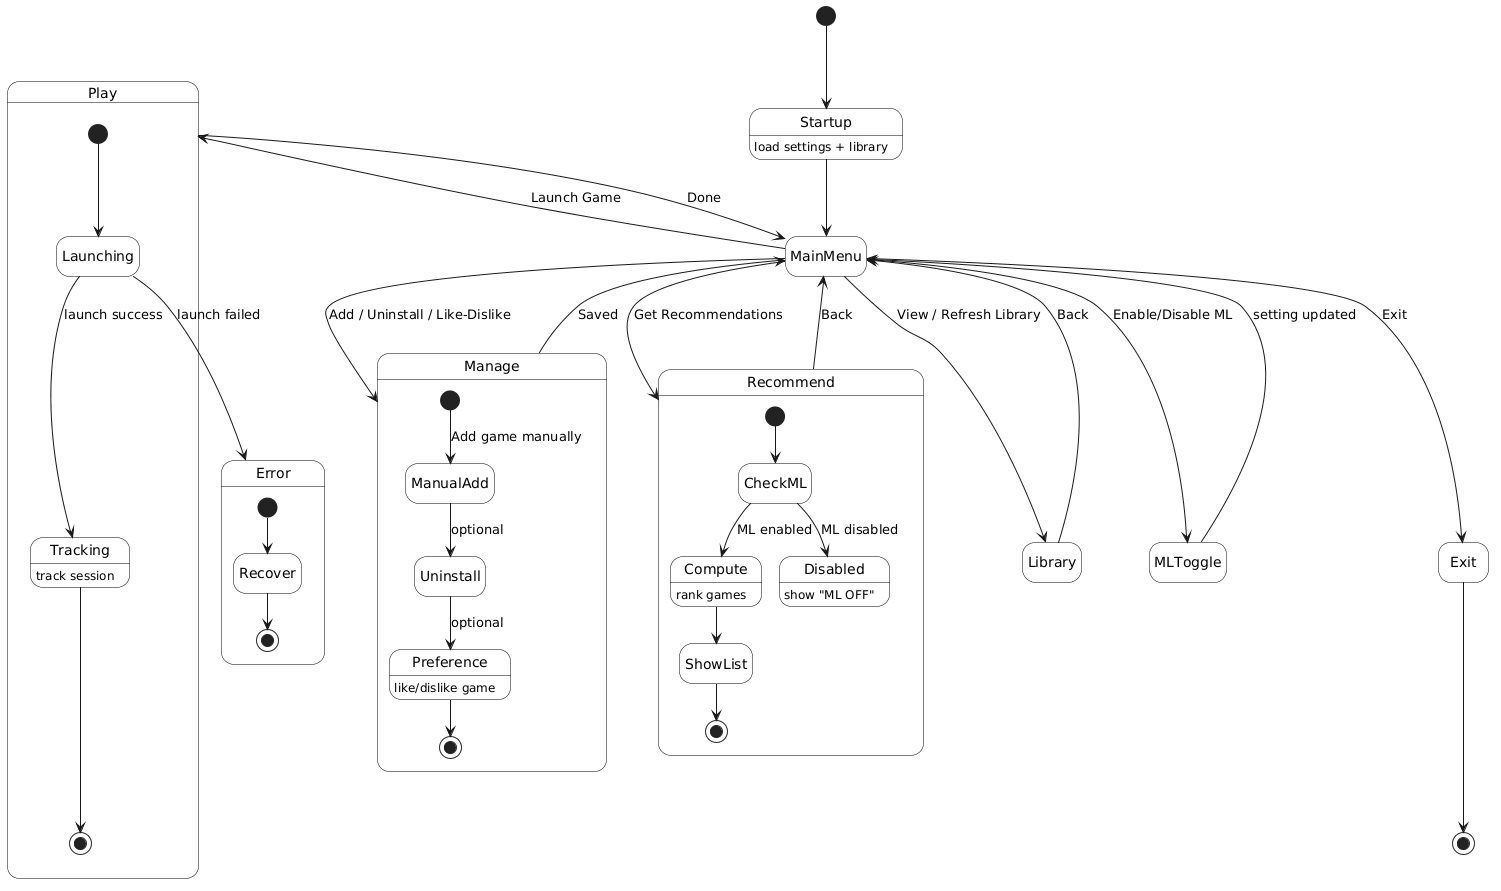
\includegraphics[angle=90, width=\textwidth]{../figures/State_diagram_compact.png}
    \caption{State Diagram (Source: By Team)}
\end{figure}

\subsection{\underline{Assumption and Dependencies}}
\begin{itemize}
    \item \textbf{Steam Installation}: The Steam client must be installed and accessible on the host machine.
    \item \textbf{Local Binaries}: User must have locally installed game binaries available for detection.
    \item \textbf{Network Connectivity}: Internet access is required for fetching external metadata via the IGDB API.
    \item \textbf{Environment Runtime}: Python runtime and all necessary machine learning libraries must be configured for the recommendation module.
    \item \textbf{System Permissions}: Appropriate administrative or user permissions are required for file system scanning and process initialization.
\end{itemize}
